% this is a comment in latex
% substitute this documentclass definition for uncommented one
% to switch between single and double column mode
\documentclass[11pt,twocolumn]{article}
%\documentclass[11pt]{article}

\usepackage{fullpage}
\usepackage{subfigure,indentfirst}

% for url
\usepackage{hyperref}
% for underlined text
\usepackage[normalem]{ulem}
% for including pdf figures
\usepackage{graphicx}
\usepackage[export]{adjustbox}
\usepackage[
backend=biber,
style=authoryear,
]{biblatex}
\addbibresource{myBib.bib}

\graphicspath{ {./images/} }

% my own versions: my_enumerate and my_itemize
\newenvironment{my_enumerate}{
  \begin{enumerate}
    \setlength{\itemsep}{1pt}
      \setlength{\parskip}{0pt}
\setlength{\parsep}{0pt}}{\end{enumerate}
}

\newenvironment{my_itemize}{
  \begin{itemize}
    \setlength{\itemsep}{1pt}
      \setlength{\parskip}{0pt}
\setlength{\parsep}{0pt}}{\end{itemize}
}

% this starts the document
\begin{document}

\title{CS87 Project Report: 
An Analysis of Parallel Sorting Algorithms}

\author{Marshall McArthur, Beluchi Okoronkwo, Ghazi Randhawa \\
Computer Science Department, Swarthmore College, Swarthmore, PA  19081}

\maketitle

\begin{abstract}
%The abstract is a brief summary of your work. It should be written to make the
%reader want to read the rest of your paper. Briefly state the basic contents
%and conclusions of your paper: the problem you are solving, why the reader
%should care about this problem, your unique solution and/or implementation,
%and the main results and and contributions of your work.

  %For writing organization resources, see my
 % CS Research and Writing Guide:
  
%\noindent {\small \url{www.cs.swarthmore.edu/~newhall/thesisguide} } 

%And, off my help pages~\cite{newhall:help} are links to other resources 
%for technical writing, including a writing style guide and information
%about Unix tools for creating and editing figures.  
Sorting tends to be used at many different levels of computer science study and implementation. It is often one of the first algorithmic processes that those who study computer science tend to learn. When it comes to parallelization of sorting, it often seems that sorting algorithms intuitively assume parallel expansions in their implementations. In other words, based on the step-by-step structure of sorting algorithms, it seems simple to take a sequential algorithm, use its general processes, and ultimately make it faster with some extra software engineering. Regretfully, the creation of parallel applications proves to be a challenge, given that they are influenced by multiple factors including architecture and application resources. Evidently, there are tradeoffs that need to be considered in parallel application implementations, with resources affecting the extent to which desired goals of parallelization can be produced. We consider sequential and parallel methods of sorting algorithms, and we keep the languages and architectures of performance testing between these implementations constant. We take these measures in order to offer a proper analysis of the effectiveness of different sorting algorithms in similar environments, being able to identify the quickest algorithm and the most scalable algorithm on $\frac{N}{P}$.


\end{abstract}


\section {Introduction} 

%The introduction is the big picture of your work: what, why, and how. It
%includes a definition of the problem you are solving, a high-level description
%of your solution including any novel techniques and results you provide, and a
%summary of the main results of your paper. In addition, motivates the problem
%you are solving (why should a reader find your work important), and describes
%your contribution to the area (this may not be applicable to your project).
%The first paragraph of the introduction should contain all of this information
%in a very high-level. Subsequent paragraphs should discuss in more detail the
%problem you are solving, your solution, and your results and conclusions.

Sorting algorithms form the basis of functionality for many large scale applications in data computation and analysis. These algorithms are often executed on shared memory processor architectures where cores share main memory with each other through caches. While processes have direct access to the same memory which implies little to small bandwidth costs, the actual implementation of some sorting algorithms under SMP systems can quickly become inefficient due to design constraints and results in high latency of communication. With this in mind, it is imperative that those wishing to maximize efficiency in their sorting algorithms must make design decisions that best align with the hardware. Additionally, although SMP architectures are the most common today, that does not mean that they are always the best hardware system for sequential or parallel sort applications. Oftentimes, algorithm structures and hardware implementations can be altered to achieve desired efficiency goals, especially for parallel algorithms.

With computing progressing at the rate it is today, it is natural to ask: what internal sorting algorithm implementations yield the most efficient solutions and under what circumstances? To answer such a question, we are investigating three internal sorting algorithm implementations in sequential and parallel applications. Each of the algorithms chosen are popular algorithms for modern computer science solutions. The algorithms examined in this paper are Odd-Even sort, RadixSort, and Bitonic Sort. Our sequential algorithms were derived from the analysis of GeeksforGeeks sequential code(\cite{Sequential-Bitonic} \cite{Sequential-oddeven}\cite{Sequential-Radix}) and they were generally well functional. These algorithms are ripe for parallelisation because they are computationally more expensive and complex than simpler sorting algorithms like bubble sort and parallelisation would allow for great savings in time and space costs.

In our solution, we juxtapose the sorting algorithms using MPI. MPI (Message Passing Interface) is a portable message passing interface that is used to create parallel programs in C or Fortran77, and is designed to work efficiently on most parallel architectures. MPI is predominantly used in conjunction with cluster systems, which employs distributed memory. MPI is the standard for parallel computing, and defines how simultaneous processes communicate and work in conjunction with each other to complete various tasks efficiently. MPI offers a defined set of routines that can be implemented with ease, allowing for developers to focus their efforts on distinct portions of the program rather than discovering ways to properly parallelize the program.
%add more about MPI 
MPI has been found to work well, and ease the strain on developers by providing simple and efficient ways to not only parallelize code, but to transform a formerly sequential program into a parallel program. 

%Here talk about why we are doing this the way we are doing it. Also talk about how we are examining the sorting algorithms along with the parallel frameworks.

This research pertains to the efficiency of MPI. Our interest lies in the speed at which OddEvenSort, RadixSort, and BitonicSort run when using this parallel framework as its means of parallelization. Does a distinct difference in runtime speed and efficiency occur when a developer uses or employs MPI for different sorting algorithms? We examine this by comparing and contrasting the three sorting algorithms while using MPI, and examining the speedup witnessed between the sequential algorithm and the parallel algorithm. Is there a distinct difference in efficiency? Does one sorting algorithm consistently beat out the others when it comes to efficiency? If so, why is that the case? These are some the questions our research wishes to explore in the examination of these sorting algorithms with MPI. 



\subsection{Odd-Even Sort}
Odd-Even Sort, is a sorting algorithm that is built for use on parallel processors. The OddEven sorting algorithm is essentially a variant of bubble sort. The algorithm is divided into two separate phases: the odd phase, and the even phase. OddEven runs until the desired array is sorted, and each iteration of the sort has both an odd and a even phase. The odd phase consist of a bubble sort of the odd indexed elements in the array, while the even phase completes a bubble sort of the even elements in the array. The sorting algorithm works by comparing the odd-even elements/pairs of adjacent elements in a list. If a pair is in the wrong place, it is then switched so that it maintains the correct sequential pattern. The following step does the same for the even/odd indexed pairs; alternating between even and odd until the entire list is sorted properly. The Odd-even sorting algorithm requires one to walk down the entire list, thus its time complexity is $O(n)$.


\subsection{RadixSort}
%We might need to go over this explanation to ensure that it is correct. 
RadixSort is an integer sorting algorithm that uses digit by digit sorting. The algorithm completes a digit by digit sort, which begins from the least significant digit and ends at the most significant digit. The algorithm sorts data by employing the use of integer keys, which it groups based on individual digits that share the same place value. This particular algorithm is often used when the records that require sorting are keyed by multiple fields. For example, if the developer wants to sort on three keys: month, day, year. Using RadixSort, one can first sort the data based on the date, then the month, and finally based on the year. The lower runtime bound for comparison based sorting algorithms (Merge Sort, Heap Sort, Quick-Sort .. etc) is $\Omega(nLogn)$. These algorithms cannot perform better than $nLogn$. Radix Sort takes $O(d*(n+b))$ time. If we define $b$ as being equal to $n$, our time complexity becomes $O(n)$. Thus, an array of integers can be sorted from a range of $1$ to $n^c$ if the numbers are represented in base $n$. 

\subsection{BitonicSort} 
Bitonic sort can be described as a classic parallel sorting algorithm. Bitonic sort mainly involves two steps. The first step involves forming a bitonic sequence. A sequence is defined as bitonic when it is first increasing and then decreasing. After completing step one, the first half of the given array is sorted in increasing order and the second half has been sorted in decreasing order. Subsequently, we compare the first element of the first half with the first element of the second half of the array; then we compare the second element of the first half with the second element of the second half and continue the process. We will only swap the elements if the value in the first half of the array is smaller. After the sorting and swapping steps we now possess two bitonic sequences in the given array. We then repeat the process within the newly created bitonic sequences, resulting in the existence of four bitonic sequences. This process will repeat until we create a bitonic sequence of size $1$. Thus, we have a $n/k$ bitonic sequences, each sequence is sorted and contains one element, leaving us with a sorted array. Bitonic sort has runtime of $O(nLog^2n)$.    


\section {Related Work}\label{relwork}
%This is an essential part of a research paper; discussing related work is a
%good way to put your work in context with other similar work, and to provide a
%way for you to compare/ contrast your work to other's work.  You should use
%feedback on the annotated bibliography from your project proposal to structure
%this section; it should be written as a re-write of your annotated bibliography
%in a single Related Work section.

Different sorting processes throughout computer science fields are necessary for proper data processing and computation. As a result, the efficiency and effectiveness of sorting algorithms have been the focus of researchers in these fields. 

\subsection{A radix sorting parallel algorithm suitable for graphic processing unit computing}
\cite{Xiao}. proposed a CPU-GPU hybrid model for minimizing the overhead that comes with increasing the data size input for Radix sorting. Additionally withing the algorithm, OpenCL as a CPU accelerator is used for quicker execution time. It is noted in their research however that their hybrid approach is subject to faults, as porting to the GPU involves transmission delay that makes the speed up gained by GPU usage not very beneficial. Their parallel algorithm is said to take $O(m({n/p}+\log{p})$ with $m$ representing their auxiliary array size, $n$ representing their data size, and $p$ representing the number of processes the parallel sort uses. This is comparable to our parallel Radix sort implementation running time, as ours is also dependent on an array (our MPI buffer) and the number of processes and data size inputs.

The results of \cite{Xiao} et al. are that radix sort speedup has a bottleneck of global memory bandwidth when performing operations. However, the algorithm attains great speedup over sequential implementation on the CPU, and generally is a good parallelization technique for improving the performance times of Radix sort. It was also noted in the article that a strictly OpenCL implementation proved to be faster than a strictly CUDA implementation, which solidifies their claims of porting slowing down potential gains from using the GPU in this environment. Cleary, there are tradeoffs when it comes to different parallel Radix sorts, which proved to be the main takeaway from this article. 

\subsection{A Comparative Study of Parallel Sort Algorithms}
Stepping slightly deeper into inter-algorithm analysis, \cite{Pasetto}. performed a comparative study of sorting algorithms, which inspired us for our own research experiments. The authors analyzed parallel implementations of Mapsort, Mergesort, and Quicksort. It is notable that they mention not including bitonic or Radix sort in their analyses, which makes our research ever more important by providing even more results of sorting algorithms' performance for comparison.

\cite{Pasetto} explains how parallel sorting algorithms can often be difficult to design, as even ones designed well on paper may not achieve the exact results intended (example Xiao et al. CUDA implementation from before). As a result, careful consideration for data and hardware must exist in these algorithms. With this in mind, the authors mention how each of the parallel algorithms they used were implemented in C++, and used C++ classes to hold immediate buffers (buffers in between computational steps) in order to decrease the overhead of huge array memory management that is often persistent in large-scale sorting computations' inputs. The results of the study found that again like Xiao et al., large memory bandwidth played a crucial role for sorting speeds. Mapsort and Mergesort were faster than Quicksort, but all the implementations gained speedup over their sequential versions. The largest takeaway from the results was that strong scalability was hard to achieve (due to the bottleneck mentioned earlier with memory) but speedup was not. In turn, more research is needed in order to internally get rid of memory bottlenecks within parallel implementations.

This research article has provided us valuable insights that when it comes to parallel sorting algorithms, the software implementation proves to be the key determinant of achieving speedup, but the hardware is what ultimately controls the level to which these sorting algorithms can extend in scalability. We will compare our findings to this research and see whether or not it aligns similarly.



%\subsection {One or more sections describing your Solution}\label{soln}
%Details of the problem you are solving Details of your solution and the
%project's implementation Even though you may have spent an enormous amount of
%time writing code, this should not include a listing of any code you wrote.
%Only if your project is about developing an algorithm or a new language, may
%code examples be appropriate here.  Discussion of how your solution solves the
%problem.
\section {Parallel Implementations}\label{relwork}
\subsection {Parallel OddEven}\label{soln}
Our  parallel  OddEvenSort  implementation  used MPI  for  thread  building  and  communication, and  was  implemented  in  C.  In comparison to the sequential version of OddEvenSort, this version allocated contiguous portions of the array to be sorted to parallel processes under the assumption that the number of processes was much smaller than the number of values in the array. Similar to the sequential version, the algorithm works under a system of rounds, with rounds being dedicated to even/odd exchanges or odd/even exchanges. However, parallel OddEven involves a local sorting step, and then a redistribution step of values between rounds before repeating the process.

To start, the program allocates each process $n/p$ data values from the array. Then, the program calls the oddevenParallel function on each process which does the following steps:
\begin{enumerate}
    \item Each process sorts locally using Quicksort.
    \item The processes assess where to share local values based on whether the round is odd or even. If the round is even, an even/odd exchange occurs. The even/odd exchange implements one of two options. If the process is even, the process then sends its locally sorted array to the process above it (process + 1). If the process is odd, the process then sends its locally sorted array to the process below it (process - 1). The send is implemented using MPI-Send, and a complimentary MPI=Recv is called to receive the sent array in a buffer. Once the processes have received the other processes local array values via the buffer correctly, the processes compare their local values with one another. For even processes, they keep the smallest half of values of the two arrays in their local array. For odd processes, they keep the largest half of the values of the two arrays in their local array. As for the odd/even exchange, the opposite for each of these steps is true. If the process is even, the process then sends its locally sorted array to the process above it (process - 1), and keeps the largest half of values of the two arrays in their local array. If the process is odd, the process then sends its locally sorted array to the process below it (process + 1) and keeps the smallest half of the values of the two arrays in their local array. 
\end{enumerate}
This algorithmic process is called within a while loop, and its iterations run so long as the number of rounds is less than the number of threads times two. This ensures that the final output has each process containing the values of the large array in order from smallest to largest.

\subsection {Parallel Radix}\label{soln}
Our parallel Radix sort implementation used MPI for thread building and communication, and was implemented in C++. Our implementation was based upon a web page about parallel Radix algorithm by \cite{Jordy}. We got stuck at the redistribution step of the algorithm and it was resolved by some insights by \cite{Parallel-Radix} implementation. The algorithm included methods from sequential Radix sort, but added in parallelization for sorting contiguous portions of the array to be sorted, and also by communicating between processes to redistribute values. These step were completed based on sequential Radix principles. The algorithm works by initiating multiple rounds of local sort, performed by each process in parallel, with a redistribution step after every round.
\includegraphics[scale=0.23]{radix sort process demo.png}

Similar to OddEven, the program starts by allocating each process its portion of $n/p$ array values. Then each process calls the radixsortParallel function. The steps of this function are as follows:
\begin{enumerate}
    \item Sort local values using countsort. Countsort takes in the local array and the exponent by which the key digit of the sorting shall be chosen (the key digit just refers to the base10 digit place by which the numbers are to be sorted, either the ones places, tens place, hundreds place, etc.). Counting sort makes a count array of size 10 and stores the counts of each base10 value from the local array into their respective buckets. The count array is then modified to store the prefix sum of the counts, or in other words each element at each index stores the sum of previous counts. Lastly there is some slight modification for sorted array output.
    \item The local count array values (with no prefix sums) of each process are shared to all other processes via an MPI-Allgather() call, which these processes receive in a buffer.
    \item For this step, each process adds up the prefix sum histogram values of all processes "left" of them (processes$<$current process). It then uses these values to determine the other processes it will share its local array values to. The sharing is done via an MPI-Isend and an MPI-Recv. The interesting part about this sharing step is that the local bucket value that is being shared and the destination process index are shared together within an array as a pair.
\end{enumerate}
This algorithmic process is called within a for loop, and repeats for however many digits there are in the largest value of the local array (for example if the number was 1000, it would run for four total times). This ensures that the values are sorted by each base10 digit, as Radix sort naturally intends. 


\subsection{ Parallel Bitonic}\label{soln}
Our parallel implementation of Bitonic sort was written in C in conjunction with MPI, much like our implementation of OddEven Sort. Our Bitonic sorting algorithm employed some of the same methods/functions we made use of in our sequential implementation. 
\begin{enumerate}
    \item The algorithm works by first spawning the threads, which then create their own arrays and populate them individually.
    \item  The threads are then paired together. Each of the threads subsequently follows the same process as the sequential Bitonic sort where they run through the array and create a Bitonic sequence. As we mentioned earlier, a sequence is defined as Bitonic, when it is first increasing and then subsequently decreasing.
    \item After finishing this step, the first half of the arrays are sorted in increasing order, while the second half is sorted in decreasing order. It is at this point that MPI truly makes itself known.
    \item The threads then pass half of their elements to another thread (either the lower or upper half's), and they receive either and increasing or decreasing sub-sequence depending on their thread number.
    \item The function then sorts this new sequence in the same manner it does when run sequentially
    \item The threads repeat this process until their entire array is sorted, finally returning a completely sorted array. 
\end{enumerate}  



\section {Results}\label{results}
%Experimental Results demonstrating/proving your solution Explain the tests you
%performed (and why) Explain how you gathered the data and details of how your
%experiments were run (any system/environment set up) Present your results
%Choose quality over quantity; the reader will not be impressed with pages and
%pages of graphs and tables, instead s/he wants to be convinced that your
%results show something interesting and that your experiments support your
%conclusions.  Discuss your results!  Explain/interpret your results (possibly
%compare your results to related work). Do not just present data and leave it up
%to the reader to infer what the data show and why they are interesting.  
\subsection{Sequential}

In order to properly contrast our parallel sorting algorithms, we needed to first identify how each of our algorithms performed when running sequentially. This information will serve as our baseline and guide us in portraying the speedup that each sorting function experienced when we modified it to run in parallel using MPI. Building from this initial frame, we proceeded to run a similar runtime test on each sorting algorithm. Our test consisted of simply increasing the size of the array that each sorting algorithm was required to parse through and recording the runtimes for those sizes. The various arrays ranged from some thousands of elements to more than a million elements that required sorting. These large sizes allow for our data to more accurately determine the capabilities of the selected sequential algorithms; resulting in more accurate data. Such large array sizes also better depict the benefits of parallel algorithms, which subsequently, allow us to more accurately determine which of our parallel implementations performs the most efficiently. The sequential test for all of the selected sorting algorithms was exported into their own CSV files, where the size of the array is paired with the runtime. We then proceeded to create a Python program that employed plotly to construct graphs based on our previous test runs. 

These were our runtime graphs for the sequential versions. We can observe in Figure \ref{fig:subim1} that the bitonic sequential algorithm has a roughly linear runtime relation with the size of inputs. In Figure \ref{fig:subim2}, the Odd-even's sequential implementation has an increasing gradient of runtime and the size input. For the Radix sort sequential implementation in Figure \ref{fig:subim3}, the run time straightens out to be a linear relationship as the size increases. Based on our initial runs of the sorting algorithms, it appears that both our Radix sort and Bitonic sort are more efficient then our OddEven sort. Additionally, Radix sort appears to be the fastest of the three sorting algorithms. Furthermore, both Bitonic sort and Radix sort display a more consistent increase in runtime as the size of the array increases. The sequential OddEven sort, however, appears to have a sharp increase in runtime when the array size reaches approximately 125k. It is possible that this difference will demonstrate itself in the parallel runs as well.     
\begin{figure}[hbt!]
\begin{subfigure}{\textwidth}
\includegraphics[width=0.9\linewidth, height=6cm]{BitonicSequential.png} 
\label{fig:subim1}
\caption{Bitonic Sequential run time tests}
\end{subfigure}
\begin{subfigure}{\textwidth}
\includegraphics[width=0.9\linewidth, height=6cm]{OddEvenSequential.png}
\label{fig:subim2}
\caption{Odd-Even Sequential runtime tests}
\end{subfigure}
\begin{subfigure}{\textwidth}
\includegraphics[width=0.9\linewidth, height=6cm]{RadixSequential.png}
\label{fig:subim3}
\caption{Radix Sequential runtime tests}
\end{subfigure}
\end{figure}

\subsection{Parallel results}
We ran our parallel test in a similar fashion. In contrast to our sequential test, our parallel test injected variation in both the size of our arrays and the number of processors being employed when sorting. Rather than keeping the number of processors consistent, we hoped to identify whether our sorting algorithms reached peak efficiency using a unique amount of processors. Furthermore, in varying the number of processors we are able to identify scalability. In doing so, we can accurately identify the number of processors that our algorithms can use before no longer seeing any improvement and whether this changes when using OddEven, Radix, or Bitonic sort. In our sequential graphs, the y-axis was defined to equal the runtime and the x-axis was defined to equal to the log(size) of the average array size of each MPI unit. Our parallel graphs were structured in much the same way. 

In Figure \ref{fig:subim4}, we can see as $\frac{N}{P}$ value increases, the runtime fluctuates widely. The purple line shows that 128 and 256 processes have mostly the highest runtimes and are somewhat constant. The smaller values of processes tend to have an increasing runtime. In Figure \ref{fig:subim5}, we can see that the largest sized values of log(N/P) tend to have the largest overhead times of communication in our algorithm. This makes intuitive sense because these processes are communicating with a larger number of processes using MPI which ballons up the costs of communication.

\begin{figure}[hbt!]
\begin{subfigure}{\textwidth}
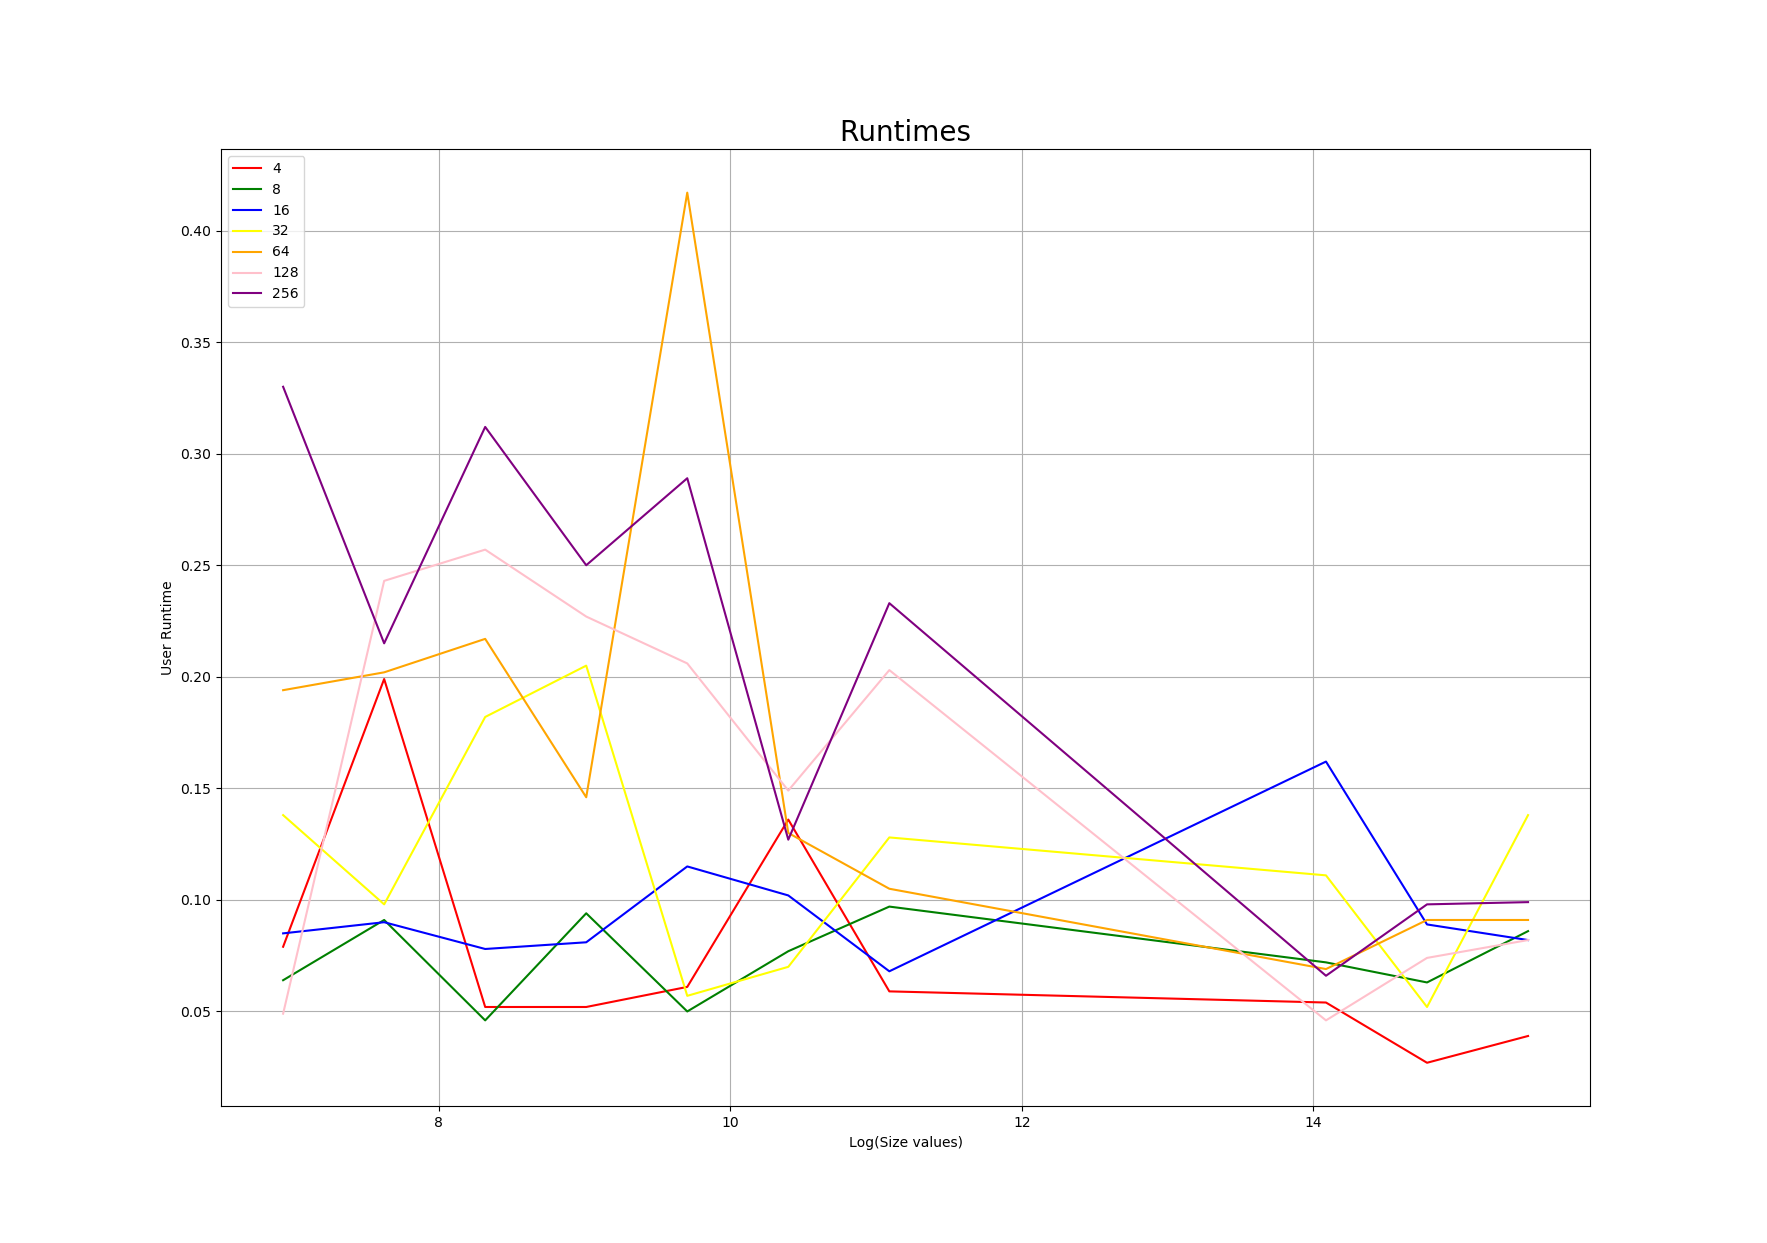
\includegraphics[width=0.9\linewidth, height=6cm]{User_runtime_final_Radix.png} 
\caption{Radix sort user runtime}
\label{fig:subim4}
\end{subfigure}
\begin{subfigure}{\textwidth}
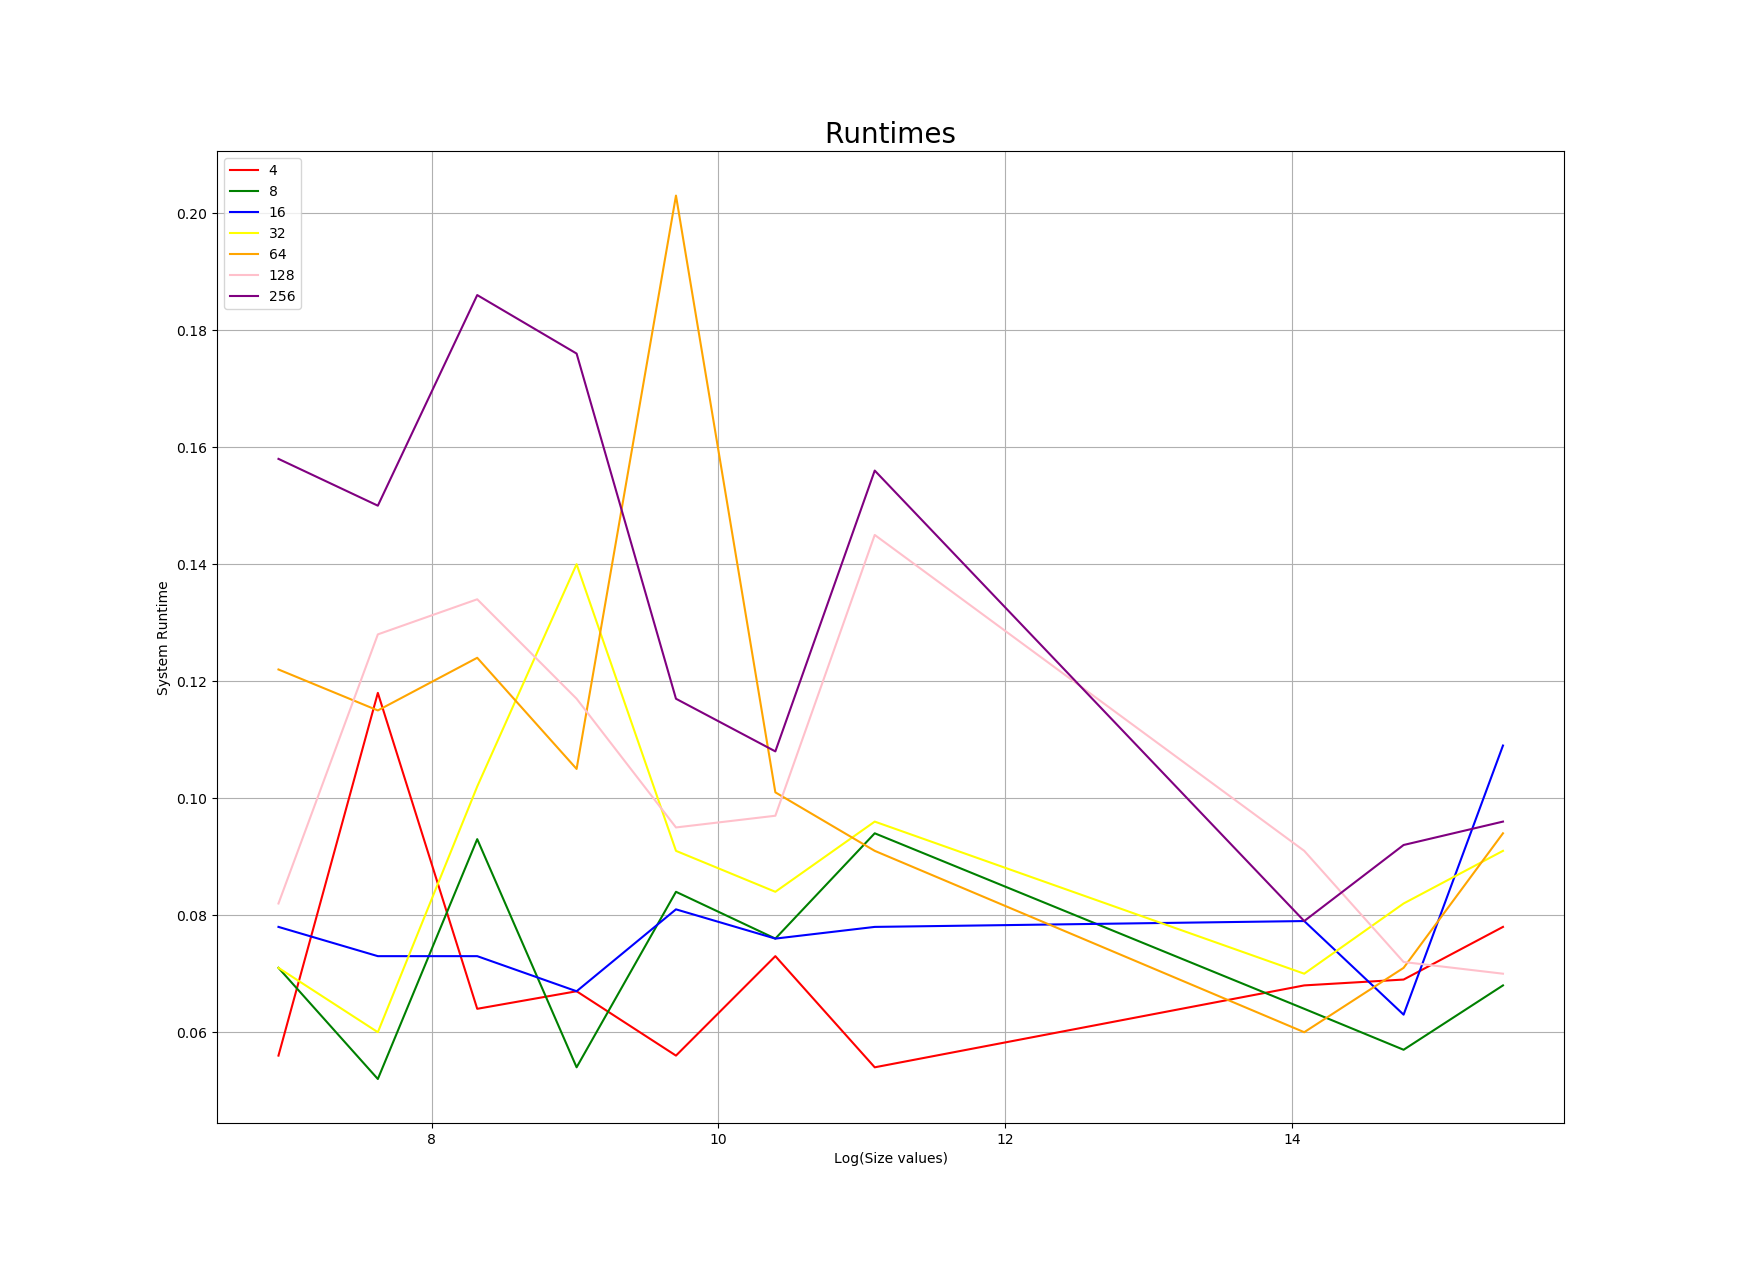
\includegraphics[width=0.9\linewidth,height=6cm]{Final_log_sys_runtime_radix.png}
\caption{Radix Sort system runtime}
\label{fig:subim5}
\end{subfigure}
\end{figure}

For our Bitonic Algorithm's Figure \ref{fig:subim6} shows that the largest number of processes tend to have the highest runtimes. These runtimes are decreasing which shows that this algorithm performs better for larger sizes. The smaller process numbers of $4,8,15,32,$ and $64$ tend to have similar runtimes. We can contrast this with our bitonic system runtime in Figure \ref{fig:subim7}which shows that most larger processes tend to have increased overhead communication costs in MPI as $\frac{N}{P}$ values increase.

\begin{figure}[hbt!]
\begin{subfigure}{\textwidth}
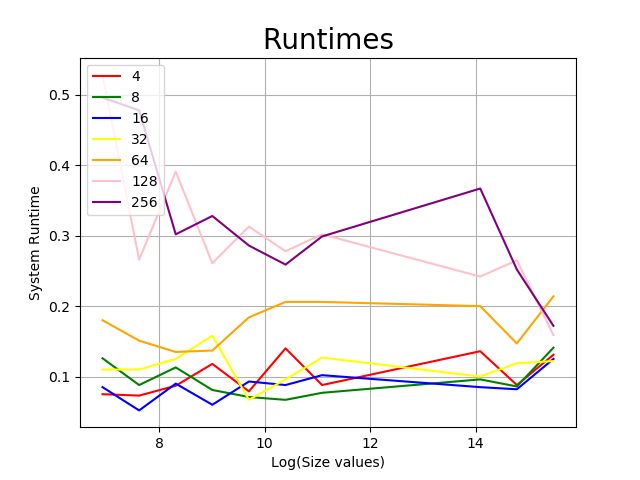
\includegraphics[width=0.9\linewidth, height=6cm]{Final_usertime_log_bitonic.png}
\caption{Bitonic sort user runtime}
\label{fig:subim6}
\end{subfigure}
\begin{subfigure}{\textwidth}
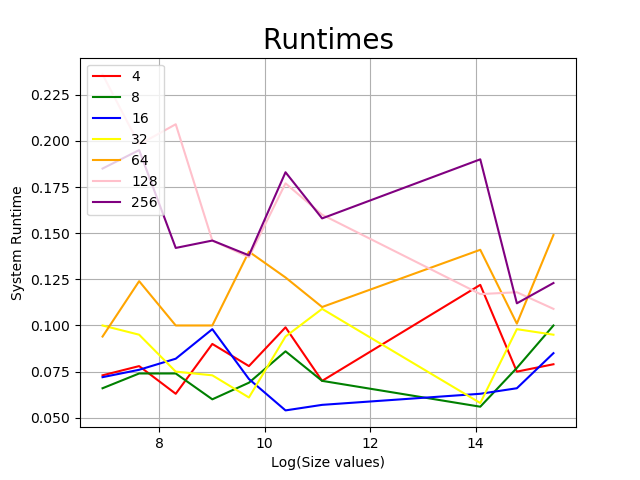
\includegraphics[width=0.9\linewidth,height=6cm]{Final_systime_log_bitonic.png}
\caption{Bitonic Sort system runtime}
\label{fig:subim7}
\end{subfigure}
\end{figure}

We observe a similar pattern with our odd-even sort. In Figure \ref{fig:subim8}, we can see that the runtime for the greater number of processes follow an overall increasing trend while the lowest number of processes have a relatively stagnant run time curves. Again, the largest number of processes in Figure \ref{fig:subim9} have the highest communication overheads, which increase over time. These larger processor curves fluctuate but overall are observed to hold an increasing pattern.

\begin{figure}[hbt!]
\begin{subfigure}{\textwidth}
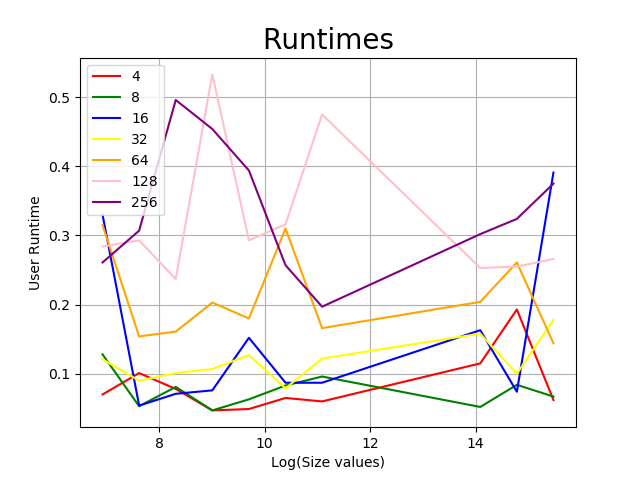
\includegraphics[width=0.9\linewidth, height=6cm]{oddeven_mpi_log_useruntime.png} 
\caption{Odd-even sort user runtime}
\label{fig:subim8}
\end{subfigure}
\begin{subfigure}{\textwidth}
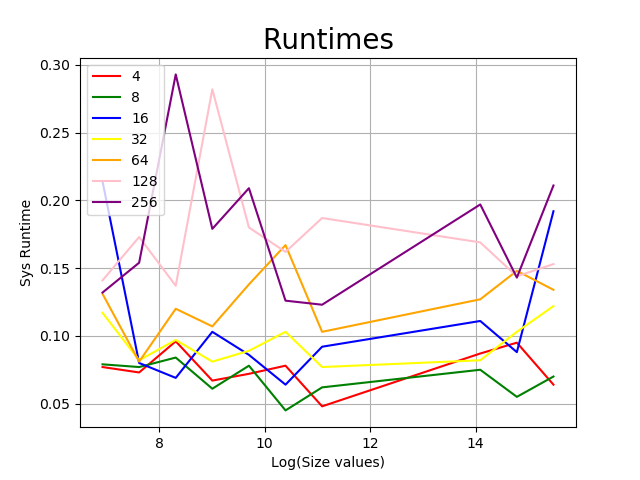
\includegraphics[width=0.9\linewidth,height=6cm]{sys_runtime_log_oddeven.png}
\caption{Odd-even Sort system runtime}
\label{fig:subim9}
\end{subfigure}
\end{figure}



    
%\subsection {Sequential Throughput}\label{soln}
%The results of the sequential runs for each sorting algorithm provided a lot of interesting insights to be considered. 

\section{Conclusions and Future Directions}\label{conc} 
The main idea of our project resides in the fact that the parallelization of sorting algorithms is a preeminent field within computer science. However, this field seems to possess many nuances that are often overlooked when considering the importance of sorted data. Parallelism has such an impact, and yet research into how parallel frameworks affect individual sorting algorithms is scarce. Our research seeks to delve deeper into the field of parallelism and its impact on sorting algorithms. Our research demonstrates that sorting algorithms when run in parallel using the same parallel method, namely MPI, handle large data in unique ways. We believe that this is just the initial step into the research into parallel sorting algorithms. In the future, it may be possible to craft certain parallel methods to work more efficiently when the knowledge of the sorting algorithm in use is at hand. Subsequently, our project has many avenues in which it can be extended. For example, future research can increase the number of sorting algorithms that are being examined. Potentially, this increase can offer a clearer picture of the efficiency of MPI and how it works in conjunction with various sorting algorithms. While we know that the runtimes of sorting algorithms differ, further research may find that the efficiency of different sorting algorithms when run in parallel can be found at differing points. Why is this the case? Does this happen due to the method by which sorting algorithms sort through arrays? If so, then similar algorithms should experience peak efficiency when using a similar number of cores, and variation between these similar algorithms ought to be reduced. Furthermore, the comparison between parallel frameworks should be implemented in the research. While some individuals have researched this topic in some capacity, it will not hurt to increase the number of parallel frameworks the sorting algorithms implement. One can include MPI, CUDA, OpenMP, and more. Increasing the number of examined frameworks enables us to identify whether certain sorting algorithms work better in conjunction with particular parallel frameworks when taken in comparison with other parallel architecture. If one is particularly ambitious, implementing a sorting algorithm that combines multiple parallel frameworks can also be done. Does a parallel sorting algorithm employing two forms of parallelization work more efficiently than a algorithm that only uses one method? There are various strategies one can adopt that would improve upon our current study, and the aforementioned avenues are a small amount of what could come next. Interestingly enough, many of the above-mentioned questions resulted from our current analysis of the selected sorting algorithms. The general question, however, can be said to be, in what ways do parallel frameworks and methods impact the efficiency of sorting algorithms, and is this impact consistent across the board? Do certain parallel methods consistently perform better than others; especially when one considers specific types of sorting algorithms?




\section{Meta-discussion}\label{meta} 
%A brief meta-discussion of your project Include two paragraphs in this section:
%Discussion of what you found to be the most difficult and least difficult parts
%of your project.  In what ways did your implementation vary from your proposal
%and why?  
%At the end of your paper is a Reference section. You must cite each paper that
%you have referenced...your work is related to some prior work.
Our project was initially about Random forests which is a part of machine learning. Unfortunately, we realized that this was a bad idea because the particular machine learning model we were to use was difficult to understand and it was difficult to include the CUDA and MPI parallelizations we were trying to introduce. Furthermore, the starter code we initially referenced was plagued with errors and did not properly compile, which increased the difficulty of our project by multiple folds. The constant run-ins with problems that we experienced up until after our midway presentation quickly brought us to a major cusp in our project. In the end, we decided to abandon our initial idea due to the aforementioned reasons, and with the support of Professor Tia Newhall, we crafted a new project that centered itself around parallel sorting algorithms.
Due to the time constraints, we knew that crafting a schedule for ourselves was an important task in ensuring the project could be completed within the remaining time. Thus, our first task as a group was to come together and decide on a timeline for our new project, which was subsequently turned into our advisor. In effect, we completed the first major step of our new project. After which, we proceeded to search for and discover sequential versions of the sorting algorithms we initially decided on. Among them were, OddEven sort, Merge sort, Bitonic sort, Radix sort, Quicksort, and Heap sort. We wished to implement both Cuda and/or MPI in all of our sorting algorithms, however, as time passed we realized that perhaps our goals were too ambitious. Thus, we decided to cut three of the initial six sorting algorithms we intended to run. Additionally, instead of implementing both CUDA and MPI, we decided that we would focus on MPI and tweak the goal of our project; we began to focus more on the efficiency of the parallel algorithms in comparison to each other rather than the contrast of MPI vs. CUDA. 
One of the most difficult parts of our project experience was deciding when to cut losses and move on in order to fulfill the greater goal of the project. We did not succeed in always making the decision in a timely manner, however, the experience has been beneficial to our growth. Furthermore, we often ran into compiler errors that continuously set back our plans. It was frustrating having our code properly written, but not being able to properly compile our work. In contrast, an easier part of our project was working with some of the more basic aspects of our sorting algorithms. Finding and tweaking our sequential code was a task that was easily accomplished, partly due to our familiarity with the sorting algorithms and another part due to the large number of references that were readily available.


% The References section is auto generated by specifying the .bib file
% containing bibtex entries, and the style I want to use (plain)
% compiling with latex, bibtex, latex, latex, will populate this
% section with all references from the .bib file that I cite in this paper
% and will set the citations in the prose to the numbered entry here
\newpage
\printbibliography
% force a page break
%\newpage 
% I want the Appendices to be single column pages
%\onecolumn
%\section{Appendices}\label{appx} 





\end{document}
